\chapter{Diseño de recursos distribuidos específicos}
\label{cap:disenyo}

%%%%%%%%%%%%%%%%%%%%%%%%%%%%%%%%%%%%%%%%%%%%%%%%%%%%%%%%%%%%%%%%%%%%%%%%%%%%%%%%
\section{Uso de la extensión aplicado a la infraestructura AppScale}
\subsection{Manifiesto de recurso distribuido}
\subsection{Fichero de roles}


%%%%%%%%%%%%%%%%%%%%%%%%%%%%%%%%%%%%%%%%%%%%%%%%%%%%%%%%%%%%%%%%%%%%%%%%%%%%%%%%
\section{Uso de la extensión aplicado a la infraestructura Torque}
\subsection{Manifiesto de recurso distribuido}
\subsection{Fichero de roles}


%%%%%%%%%%%%%%%%%%%%%%%%%%%%%%%%%%%%%%%%%%%%%%%%%%%%%%%%%%%%%%%%%%%%%%%%%%%%%%%%
\section{Uso de la extensión aplicado a la infraestructura web de tres niveles}

[Revisar]\\

Una típica arquitectura de servicios web consta de al menos tres niveles: balanceo de carga, servidores web y base de datos. Cada uno de estos niveles está compuesto por al menos un elemento clave: el balanceador de carga, el servidor web y el servidor de base de datos, respectivamente. El balanceador de carga es el punto de entrada al sistema y el que se encarga, como su nombre indica, de repartir las peticiones de los clientes a los distintos servidores web. Los servidores web se encargan de servir las páginas web a los clientes y para ello, dependiendo de las peticiones que hagan los clientes, podrán leer o almacenar información en la base de datos. Para manipular dicha información los servidores web tendrán que comunicarse con el servidor de base de datos, que es el que hará efectiva la lectura y modificación de la información. La arquitectura puede complicarse añadiendo más niveles y añadiendo más elementos a los niveles existentes.\\

\begin{figure} [!htbp]
  \centering
  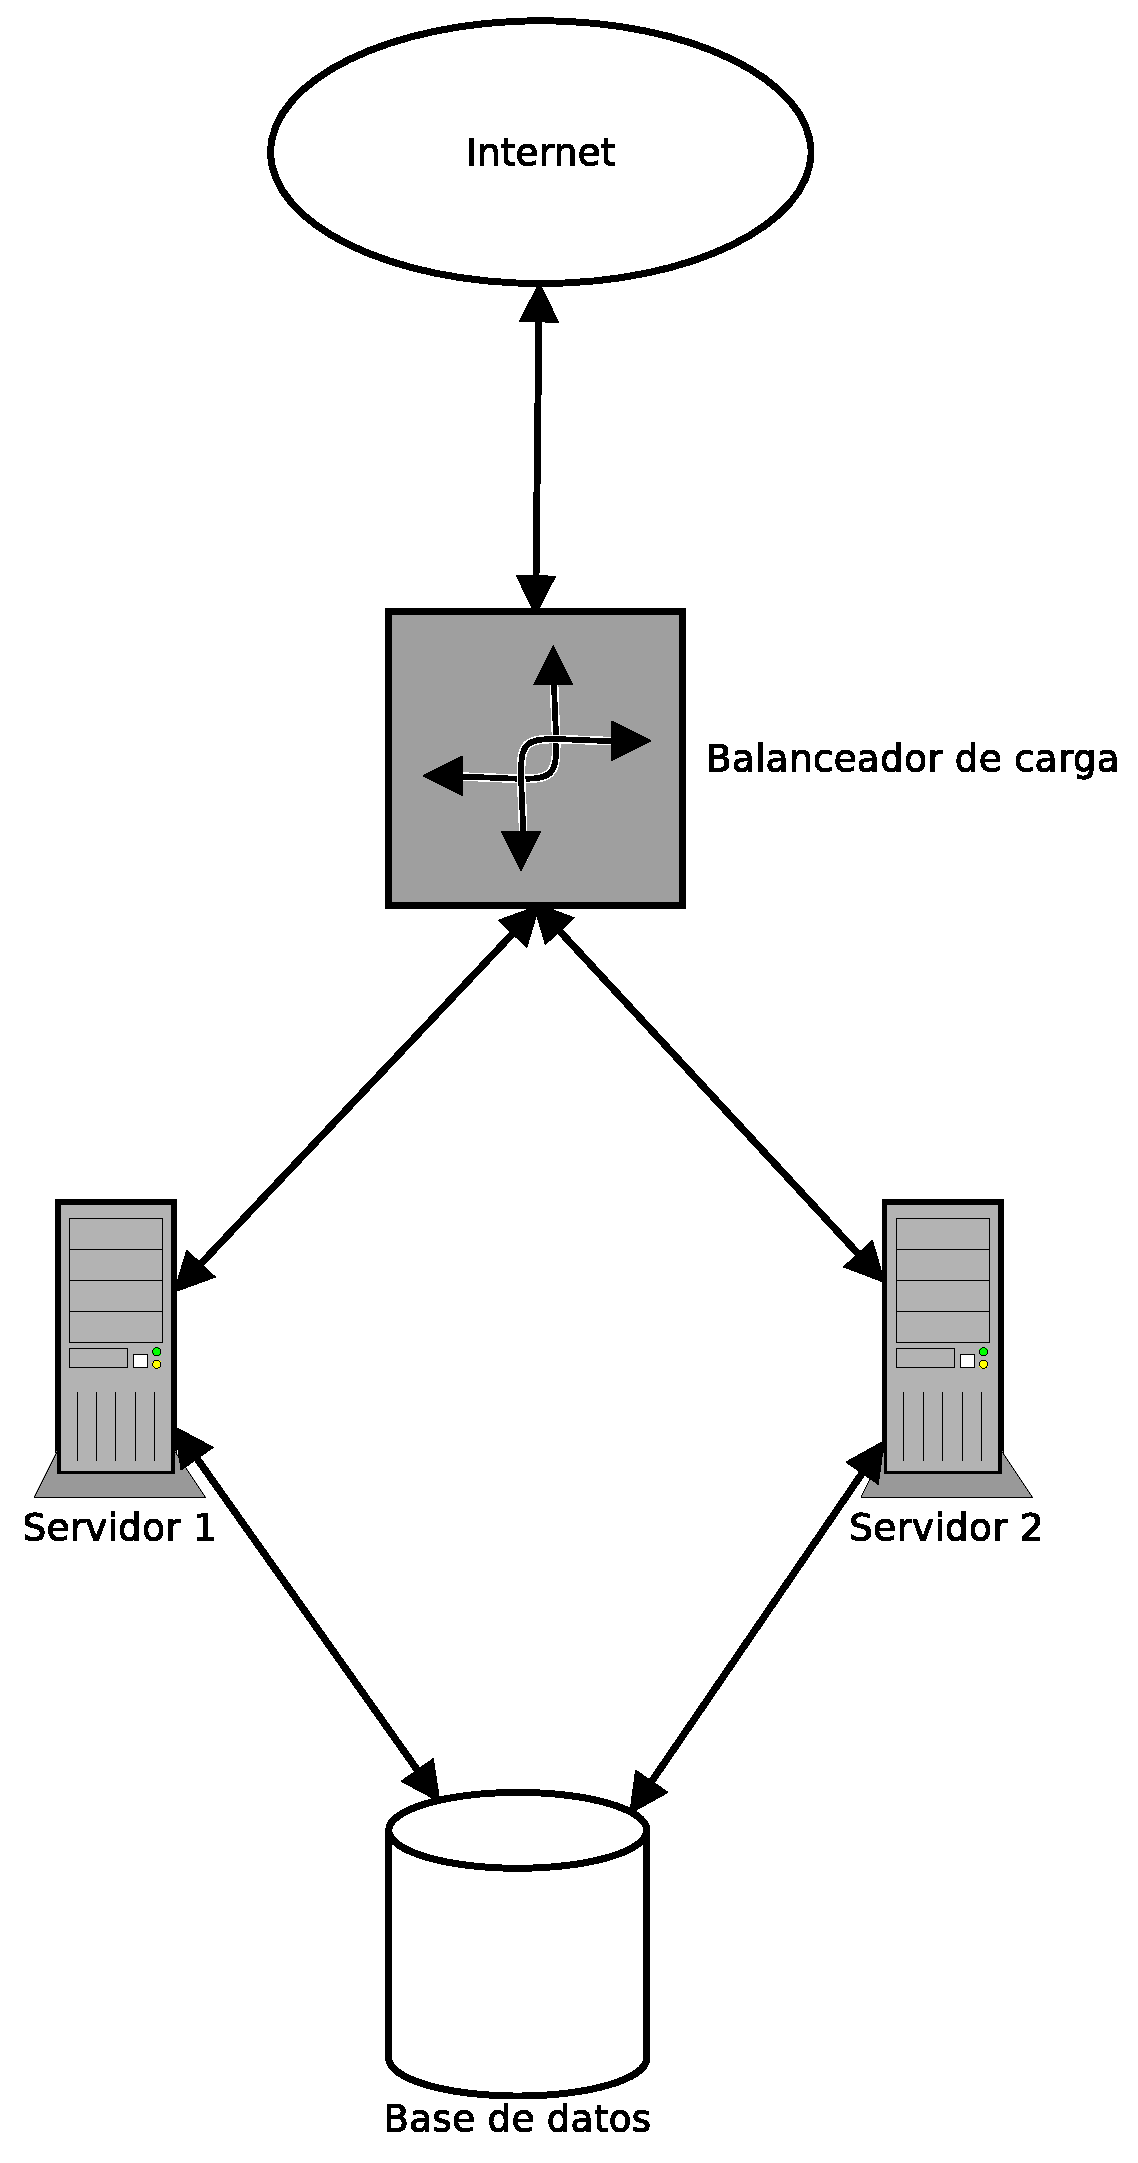
\includegraphics[width=0.5\textwidth]{figuras/Arquitectura_web2.eps}
  \caption{Arquitectura web de tres niveles.}
\label{figure:arquitectura-web}
\end{figure}

Para demostrar la validez del modelo desarrollado, además de AppScale también se puede controlar una infraestructura de servicios web. En el ejemplo se ha validado una arquitectura que consta de un balanceador de carga, dos servidores web y un servidor de bases de datos. Como balanceador de carga se ha usado nginx y como servidor de base de datos se ha usado MySQL. La creación de la página web se ha hecho usando el framework Sinatra sobre el servidor web WEBrick. Todos ellos corren sobre máquinas con sistema operativo Ubuntu.\\

\subsection{Manifiesto de recurso distribuido}

La sintaxis en el metamanifiesto es fundamentalmente similar a la utilizada en el ejemplo de AppScale: el único campo que cambia sustancialmente es el type, que pasa de tener valor \texttt{appscale} a tener valor \texttt{web}. El resto de campos se comportan como lo hacían en el ejemplo de AppScale: el campo file contiene el fichero de descripción de roles, el campo images contiene los discos duros de las máquinas virtuales, el campo domain contiene el fichero de descripción de la máquina virtual, el campo pool contiene el conjunto de máquinas físicas a usar y el campo ensure contiene el estado en el que queremos que quede el cloud.

\begin{lstlisting}
cloud {'mycloud':
   type    => "web",
   file    => "/etc/puppet/modules/cloud/files/web-simple.yaml",
   images  => ["/var/tmp/dceresuela/lucid-web.img", "/var/tmp/dceresuela/lucid-db.img"],
   domain  => "/etc/puppet/modules/cloud/files/mycloud-template.xml",
   pool    => ["155.210.155.70"],
   ensure  => running,
}
\end{lstlisting}

\subsection{Fichero de roles}

El contenido del fichero de especificación de roles sí que poseerá valores distintos a los que tenía el ejemplo de AppScale ya que estamos describiendo una arquitectura distribuida distinta. Los nuevos roles que pueden desempeñar las máquinas son:
\begin{description}
\item[\texttt{balancer}] La máquina que desempeñará el rol de balanceador de carga.
\item[\texttt{server}] La lista de máquinas que desempeñarán el rol de servidor web.
\item[\texttt{database}] La máquina que desempeñará el rol de servidor de base de datos.
\end{description}

Un ejemplo completo del fichero de especificación de roles tendría un contenido similar a éste:
\begin{yamlcode}
--- 
:balancer: 155.210.155.175
:server:
- 155.210.155.73
- 155.210.155.178
:database: 155.210.155.177
\end{yamlcode}



%%% Tests
%Tests
%\begin{rubycode}
%class MAC_Address
%   
%   attr_reader :mac
%   
%   def initialize(value=nil)
%      @mac = value ? value: "52:54:00:00:00:00"
%   end
%   
%   
%end
%\end{rubycode}
